\documentclass[12pt]{article} % This command is used to set the type of document you are working on such as an article, book, or presenation

\usepackage[margin=1in]{geometry} % This package allows the editing of the page layout. I've set the margins to be 1inch. 
\usepackage{datetime}

\usepackage{amsmath, amsfonts}  % The first package allows the use of a large range of mathematical formula, commands, and symbols.  The second gives some useful mathematical fonts.

\usepackage{graphicx}  % This package allows the importing of images


\begin{document}

\begin{center}
    \Large{
        \textbf{Reading Report:}
        Application of Catalan Numbers and the Lattice
Path Combinatorial Problem in Cryptography
    }
    
    \vspace{5pt}
        
    \normalsize{
        GEOFF YOERGER

        \usdate
        \formatdate{7}{5}{2021}
    }
    
    \vspace{15pt}

    \subsection*{Abstract}

    The paper analyzes the properties of Catalan numbers with respect to the Lattice Path encryption scheme in cryptography. The encryption/decryption keys are Catalan-keys, which are a subset of numbers with a property that is synonomous with a counting ability of the Catalan numbers proper.
\end{center}
    
\section{Introduction} 

The subject of the paper covers the use of Catalan-key numbers as a form of cryptographic text encryption.  This is performed utilizing the core properties of Catalan-key numbers, in a method called the Lattice Path Problem.  The papers also covers related work and a statistical analysis according to NIST's guidelines on cryptographic soundness;  These will not be covered in this summary.

\section{Properties of Catalan Numbers} 

\subsection{Catalan Numbers}

Catalan numbers are defined as

$$
C_n = \frac{(2n)!}{(n+1)!n!} = \frac{1}{n+1} {2n \choose n}
$$

Let $B = \{0, 1\}$ be a binary alphabet.

\subsection{Catalan-key numbers and Dyke words}

Catalan-key numbers are defined as numbers $c$ where

\begin{align*}
    c = (X_1 X_2 \cdots X_n)_2, & \; \; \; X_i \in B \\
    h(X_1 X_2 \cdots X_i) \geq 0, & \; \; \;  1 \leq i \leq 2n-1 \\
    h(X_1 X_2 \cdots X_n) = 0 & \\
\end{align*}

where $h: B^n \to \mathbb{N}$ is a mapping where

\begin{align*}
    h(0) &= 1 \\
    h(1) &= -1 \\
    h(X_1 X_2 \cdots X_n) &= \sum_{i=1}^{n} h(X_i) \\
\end{align*}

In other words, Catalan-key numbers are numbers whose binary representations are isomorphic to Dyke words.

Dyke words are words from the alphabet consisting of one left bracket and one right bracket, where all brackets are properly paired and nested. For example, and the 6-length Dyke words are:
\begin{enumerate}
    \item "[[[]]]"
    \item "[][[]]"
    \item "[][][]"
    \item "[[]][]"
    \item "[[][]]"
\end{enumerate}


By definition, the $n$-th Catalan number $C_n$ counts the number of total Dyke words of length $2n$, and because of the isomorphism between Catalan-keys and Dyke words, $C_n$ also counts the number of Catalan-keys with $2n$ bit long representations.  Hence, their name.

\section{Lattice Path Combinatorial Problem} 

The Lattice path combinatorial problem deals with the calculations of the number of paths through a $n x n$ lattice space, from point $(0,0)$ to point $(n,n)$. 

Here, we restrict movement across the diagonal line connecting the start and end points, and individual movement steps are only allowed to come from the set $\{(0,+1), (+1,0)\}$, in other words, the only possible movements are one unit right, or one unit up.

A common application of catalan numbers is showing that $C_n$ counts the total number of possible paths in such a $n x n$ lattice grid.

\subsection{Application of Catalan-key}

It follows that each $2n$-bit catalan-key uniquely represents each possible path in the lattice grid. $1$s denote movement one unit right, $0$s denote one movement up.

The restriction $ h(X_1 X_2 \cdots X_i) \geq 0$ ensures that the cummulative number of right movements is always greater than or equal to the number of up movements and any point in the path, this ensures the path never crosses the diagonal.

The restriction $h(X_1 X_2 \cdots X_n) = 0$ ensures the final endpoint of the path is $(n,n)$.

\section{The encryption scheme}

The idea presented in the paper is that these lattice paths are applicible to designate a way to encrypt a plaintext into a ciphertext by use of swapping character locations based on the bit patterns in Catalan-keys.

\subsection{The algorithm}

Using a $2n$-bit Catalan key, and an arbitrary plaintext.

\begin{enumerate}
    \item Expand the binary representation of the Catalan-key into a boolean array $A$ of length $2n$, where $A[n]$ is true if the $n$-th bit is $1$.
    \item Split the plaintext into $2n$-length segments
    \item For each segment \begin{enumerate}
            \item Make a LIFO Stack
            \item For i = 0..2n \begin{enumerate}
                    \item If $A[i]$, Pop the front character of the plaintext into the stack, this is analogous to a "right movement"
                    \item Else, Pop the top of the stack onto the end of the ciphertext, analogous to a "up movement"
            \end{enumerate}
        \item Output the encrypted segment
    \end{enumerate}
\end{enumerate}

My description of the algorithm does not match specifically the algorithm described in the paper, which uses fixed length arrays for the plaintext and ciphertext, while manually tracking the indexes into both.  Using a stack works to simplify understanding.

The properties of Catalan-keys ensure that the same number of characters will be pushed onto the stack as popped off, and that whenever a pop occurs, the stack will be not empty.

The execution of this process is completely deterministic, so decryption simply works backwards given a cipertext and key to recover the plaintext.

The algorithm can be performed on arbitrary alphabets, for example, in the encrytion of english characters, the plaintext can be first converted to its binary representation, and the binary string manipluated as above to achieve an encryption scheme whose result is far less recognizable.

\pagebreak

\subsection{An example}

Taken from the paper.

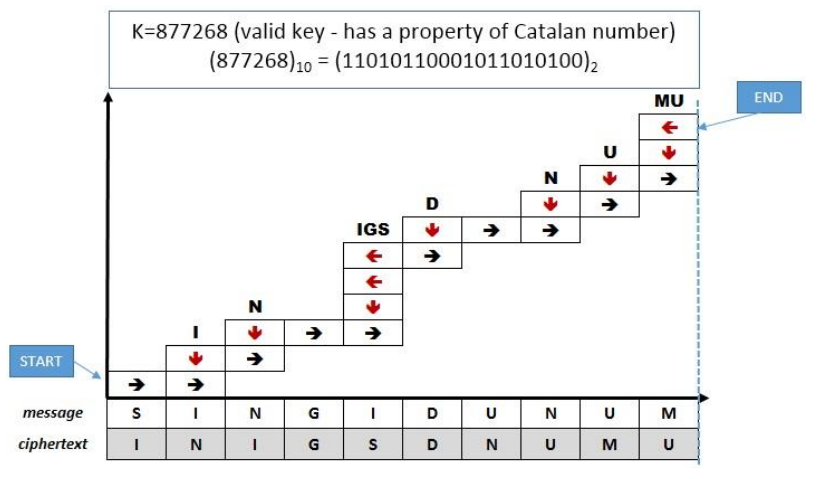
\includegraphics[width=\textwidth]{path}

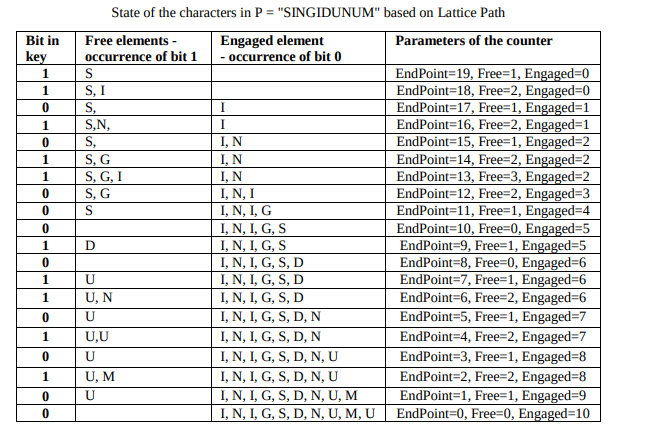
\includegraphics[width=\textwidth]{chart}

\section{Conclusion} 

This paper showed how Catalan-key numbers can be used in encryption schemes.  The core properties of Catalan-key numbers ensured the algorithms possible operation.  The parameters in the algorithm are also variable to ensure a wide execution space (key size, input representation)

However, crytographic viability was not tested, so this appeared to be mostly a proof of concept for inspiring further work.

\section{Source}

Saračević, Muzafer, Saša Adamović, and Enver Biševac. "Application of Catalan numbers and the lattice path combinatorial problem in cryptography." Acta Polytechnica Hungarica 15.7 (2018): 91-110.
    
\end{document}
